%%%%%%%%%%%%%%%%%%%%%%%%%%%%%%%%%%%%%%%%%%%%%%%%%%%%%%%%%%%%
%%% ELIFE ARTICLE TEMPLATE
%%%%%%%%%%%%%%%%%%%%%%%%%%%%%%%%%%%%%%%%%%%%%%%%%%%%%%%%%%%%
%%% PREAMBLE 
\documentclass[9pt,lineno]{elife}
% Use the onehalfspacing option for 1.5 line spacing
% Use the doublespacing option for 2.0 line spacing
% Please note that these options may affect formatting.
% Additionally, the use of the \newcommand function should be limited.

%\usepackage[version=4]{mhchem}
\usepackage{float}


%%%%%%%%%%%%%%%%%%%%%%%%%%%%%%%%%%%%%%%%%%%%%%%%%%%%%%%%%%%%
%%% ARTICLE SETUP
%%%%%%%%%%%%%%%%%%%%%%%%%%%%%%%%%%%%%%%%%%%%%%%%%%%%%%%%%%%%
\title{Provenance, Open-Source, Reproducibility \& Modularity
\newline \textnormal{Best practices for computational sciences in the context of kinase pharmacology}}

\author[1,3\authfn{1}]{Jaime Rodr\'{i}guez-Guerra}
\author[1,3\authfn{1}]{Talia B. Kimber}
\author[1,2,3]{David/Corey/Michael/Jess/Ben/?}
\author[1,2\authfn{2}*]{Andrea Volkamer}
\author[3*]{John D. Chodera}

\affil[1]{\textit{In silico} Toxicology and Structural Bioinformatics, Institute of Physiology, Charit\'e-Universit\"atsmedizin Berlin, Charit\'eplatz 1, 10117, Berlin, Germany}
\affil[2]{Data Driven Drug Design, Saarland University, Saarbrücken, Germany}
\affil[3]{Computational and Systems Biology Program, Sloan Kettering Institute, Memorial Sloan Kettering Cancer Center, New York, NY 10065}

\corr{andrea.volkamer@cs.uni-saarland.de}{AV}
\corr{john.chodera@choderalab.org}{JDC}


%\contrib[\authfn{1}]{These authors contributed equally to this work}
%\contrib[\authfn{2}]{These authors also contributed equally to this work}

%%%%%%%%%%%%%%%%%%%%%%%%%%%%%%%%%%%%%%%%%%%%%%%%%%%%%%%%%%%%
%%% ARTICLE START
%%%%%%%%%%%%%%%%%%%%%%%%%%%%%%%%%%%%%%%%%%%%%%%%%%%%%%%%%%%%

\begin{document}

\maketitle

\begin{abstract}

\end{abstract}


\section{Introduction}
% \section{Methods and Materials}
\subsection{The OpenKinome initiative}
The OpenKinome initiative aims to leverage the increasingly available bioactivity data and scalable computational resources to perform kinase-centric drug design in the context of structure-informed machine learning and free energy calculations.

\subsection{The goals}
Kinases are a well-studied group of proteins due to their important role in cancer and other diseases~\cite{kooistra_2017_annualreports}. As a result, there is an abundance of data waiting to be used in computational experiments such as machine learning. The KinoML package was created for this purpose; the name itself is a portmanteau of "kinases" and "machine learning".

An underlying assumption is that higher quality data would allow to build models with improved prediction accuracy. Eventually, the aim is to build structure-informed models that can benefit from both machine learning and free energy calculations.

However, to reach these goals, baseline models must be established and finding a way to iterate and improve in reproducible and comparable ways is essential. This calls for the following pillars:

\begin{description}
\item[Robust and extensible object models:] Regardless the source, all the data used in training, evaluation and testing must be represented in the same way, so it can be compared and reused in reliable ways.
\item[Guaranteed provenance:] Every run must be logged and every input dataset should be versioned, archived and deposited for long-term availability. If an experiment needs to be debugged, it can be run again, no matter where or when or by whom. This leads to:
\item[Reproducible pipelines, down to the bit:] Automated workflows will deterministically recreate the same models given the same input configuration data.
\end{description}

Mention FAIR (Findability, Accessibility, Interoperability, and Reusability)~\cite{Wilkinson_2016_scientificdata} principles?


\begin{figure}
\centering
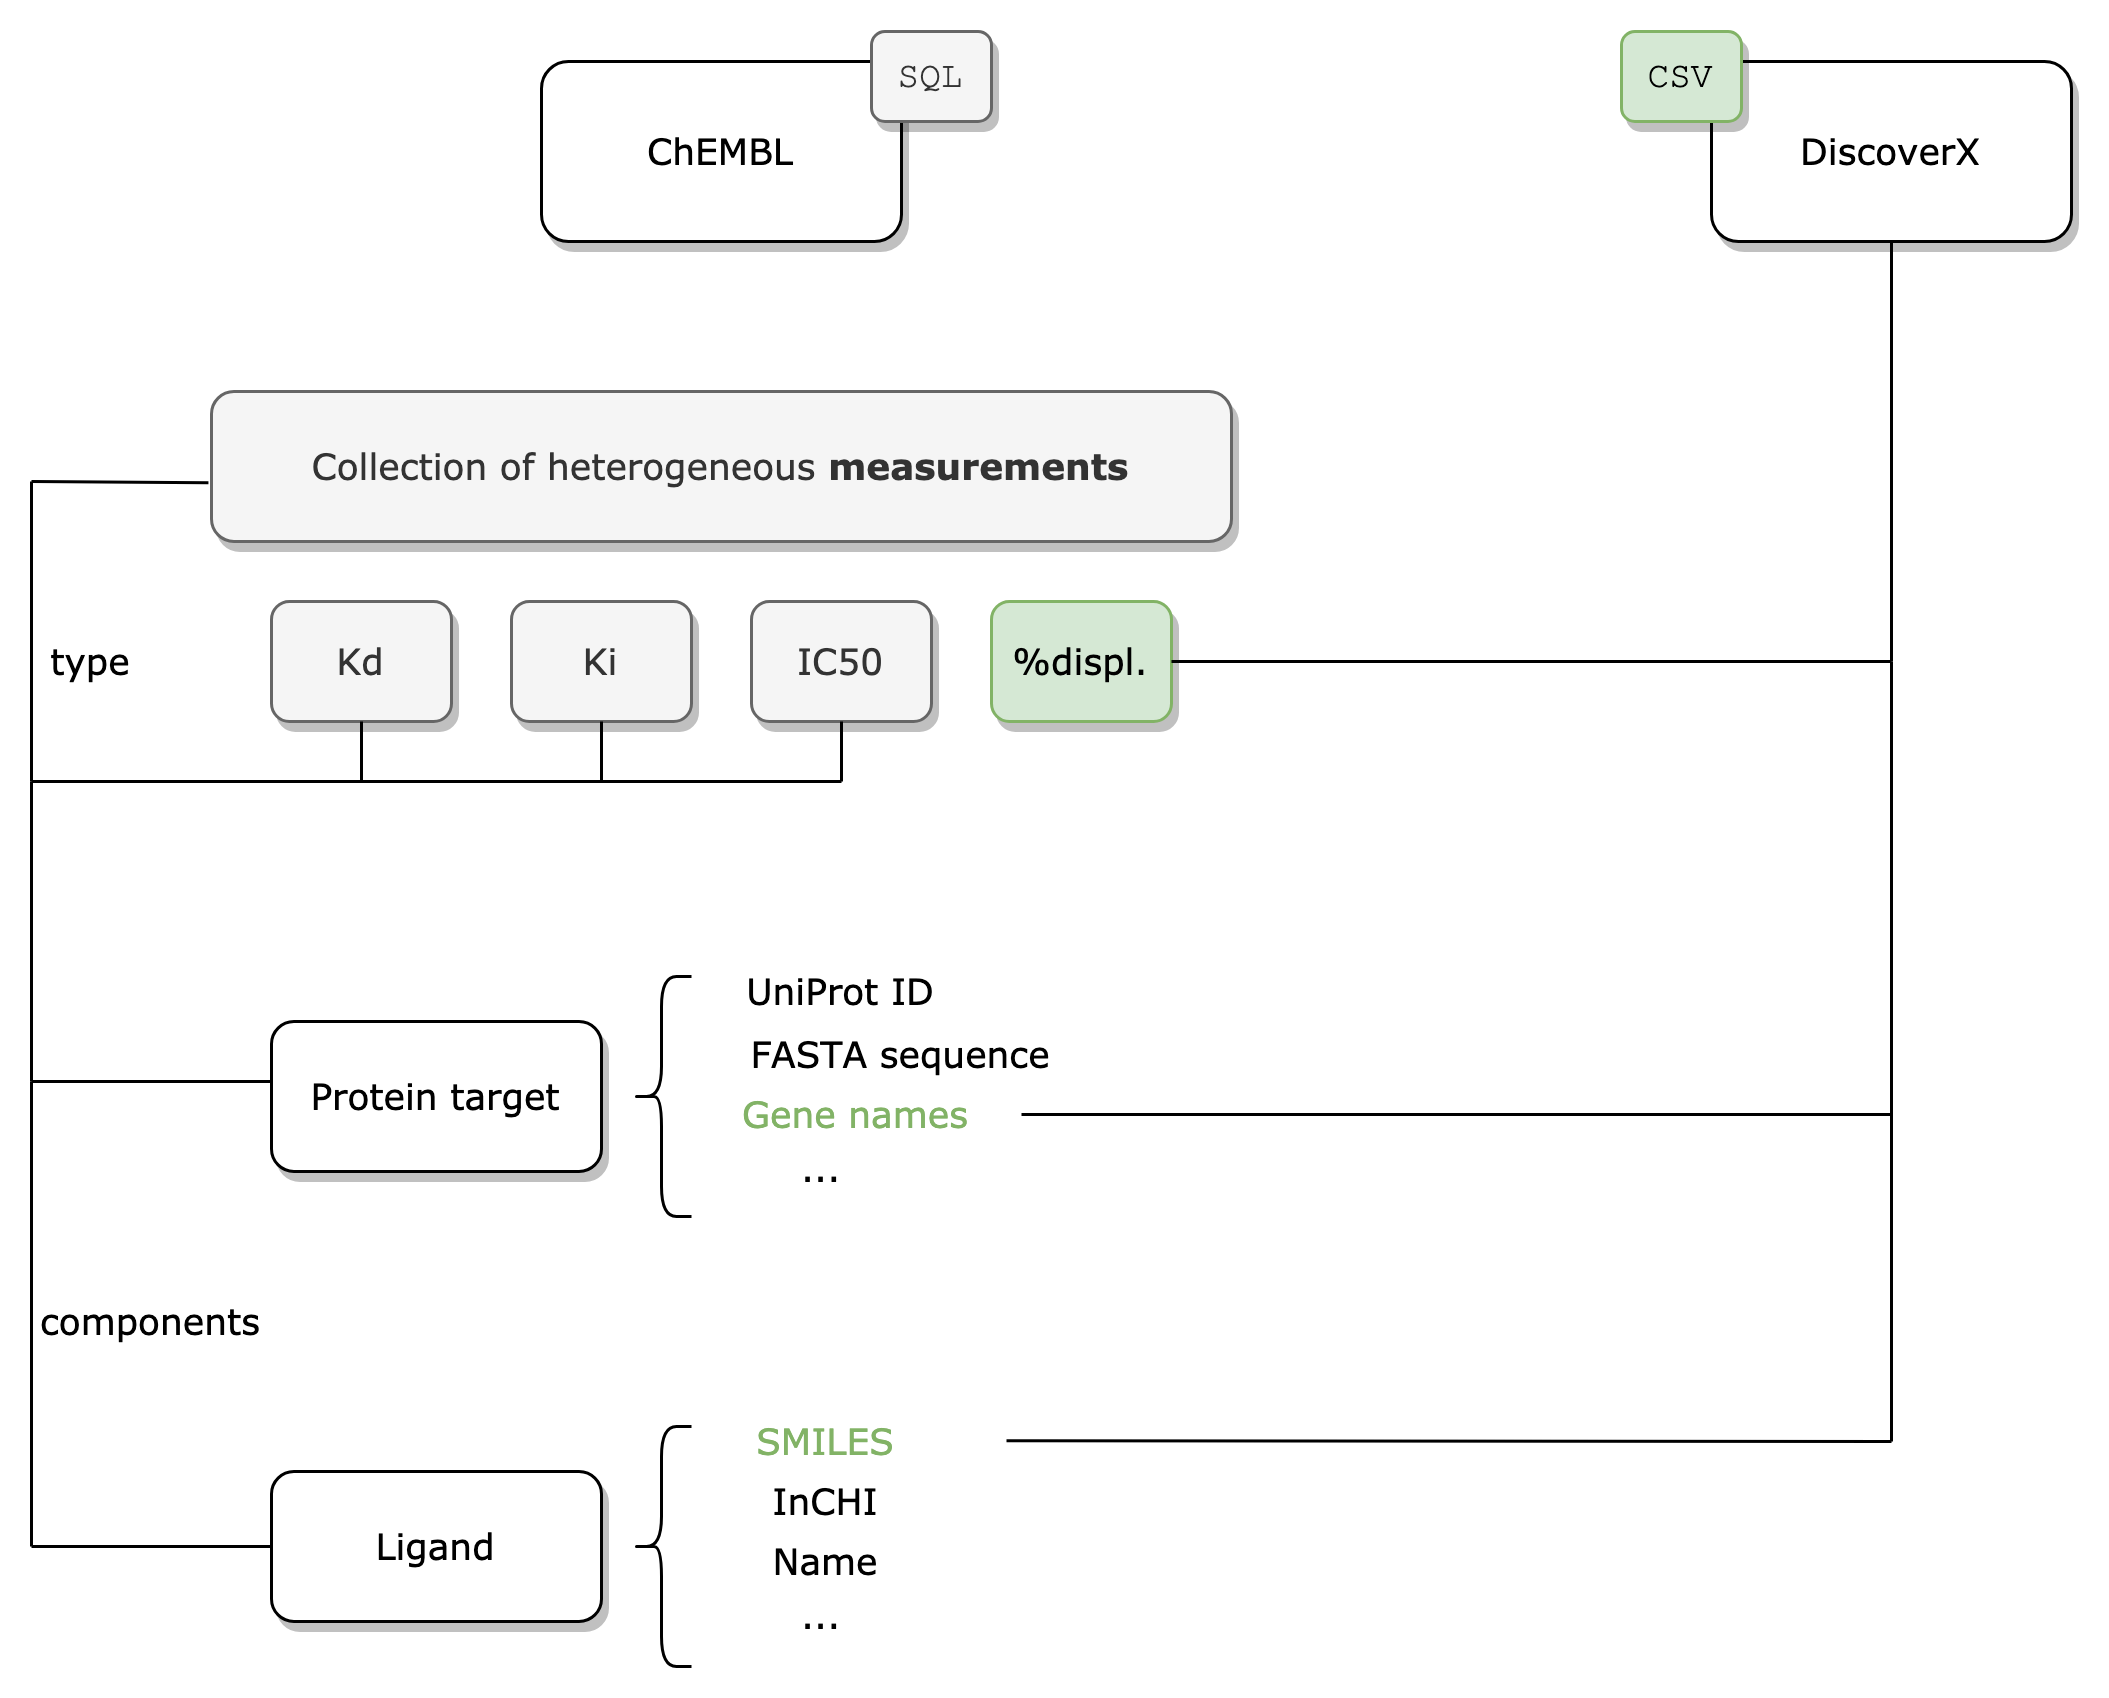
\includegraphics[width=0.5\linewidth]{figures/kinodata.png}
\caption{\textbf{Raw data.} Add.}
\label{fig:kinodata}
\end{figure}

\begin{figure}
\centering
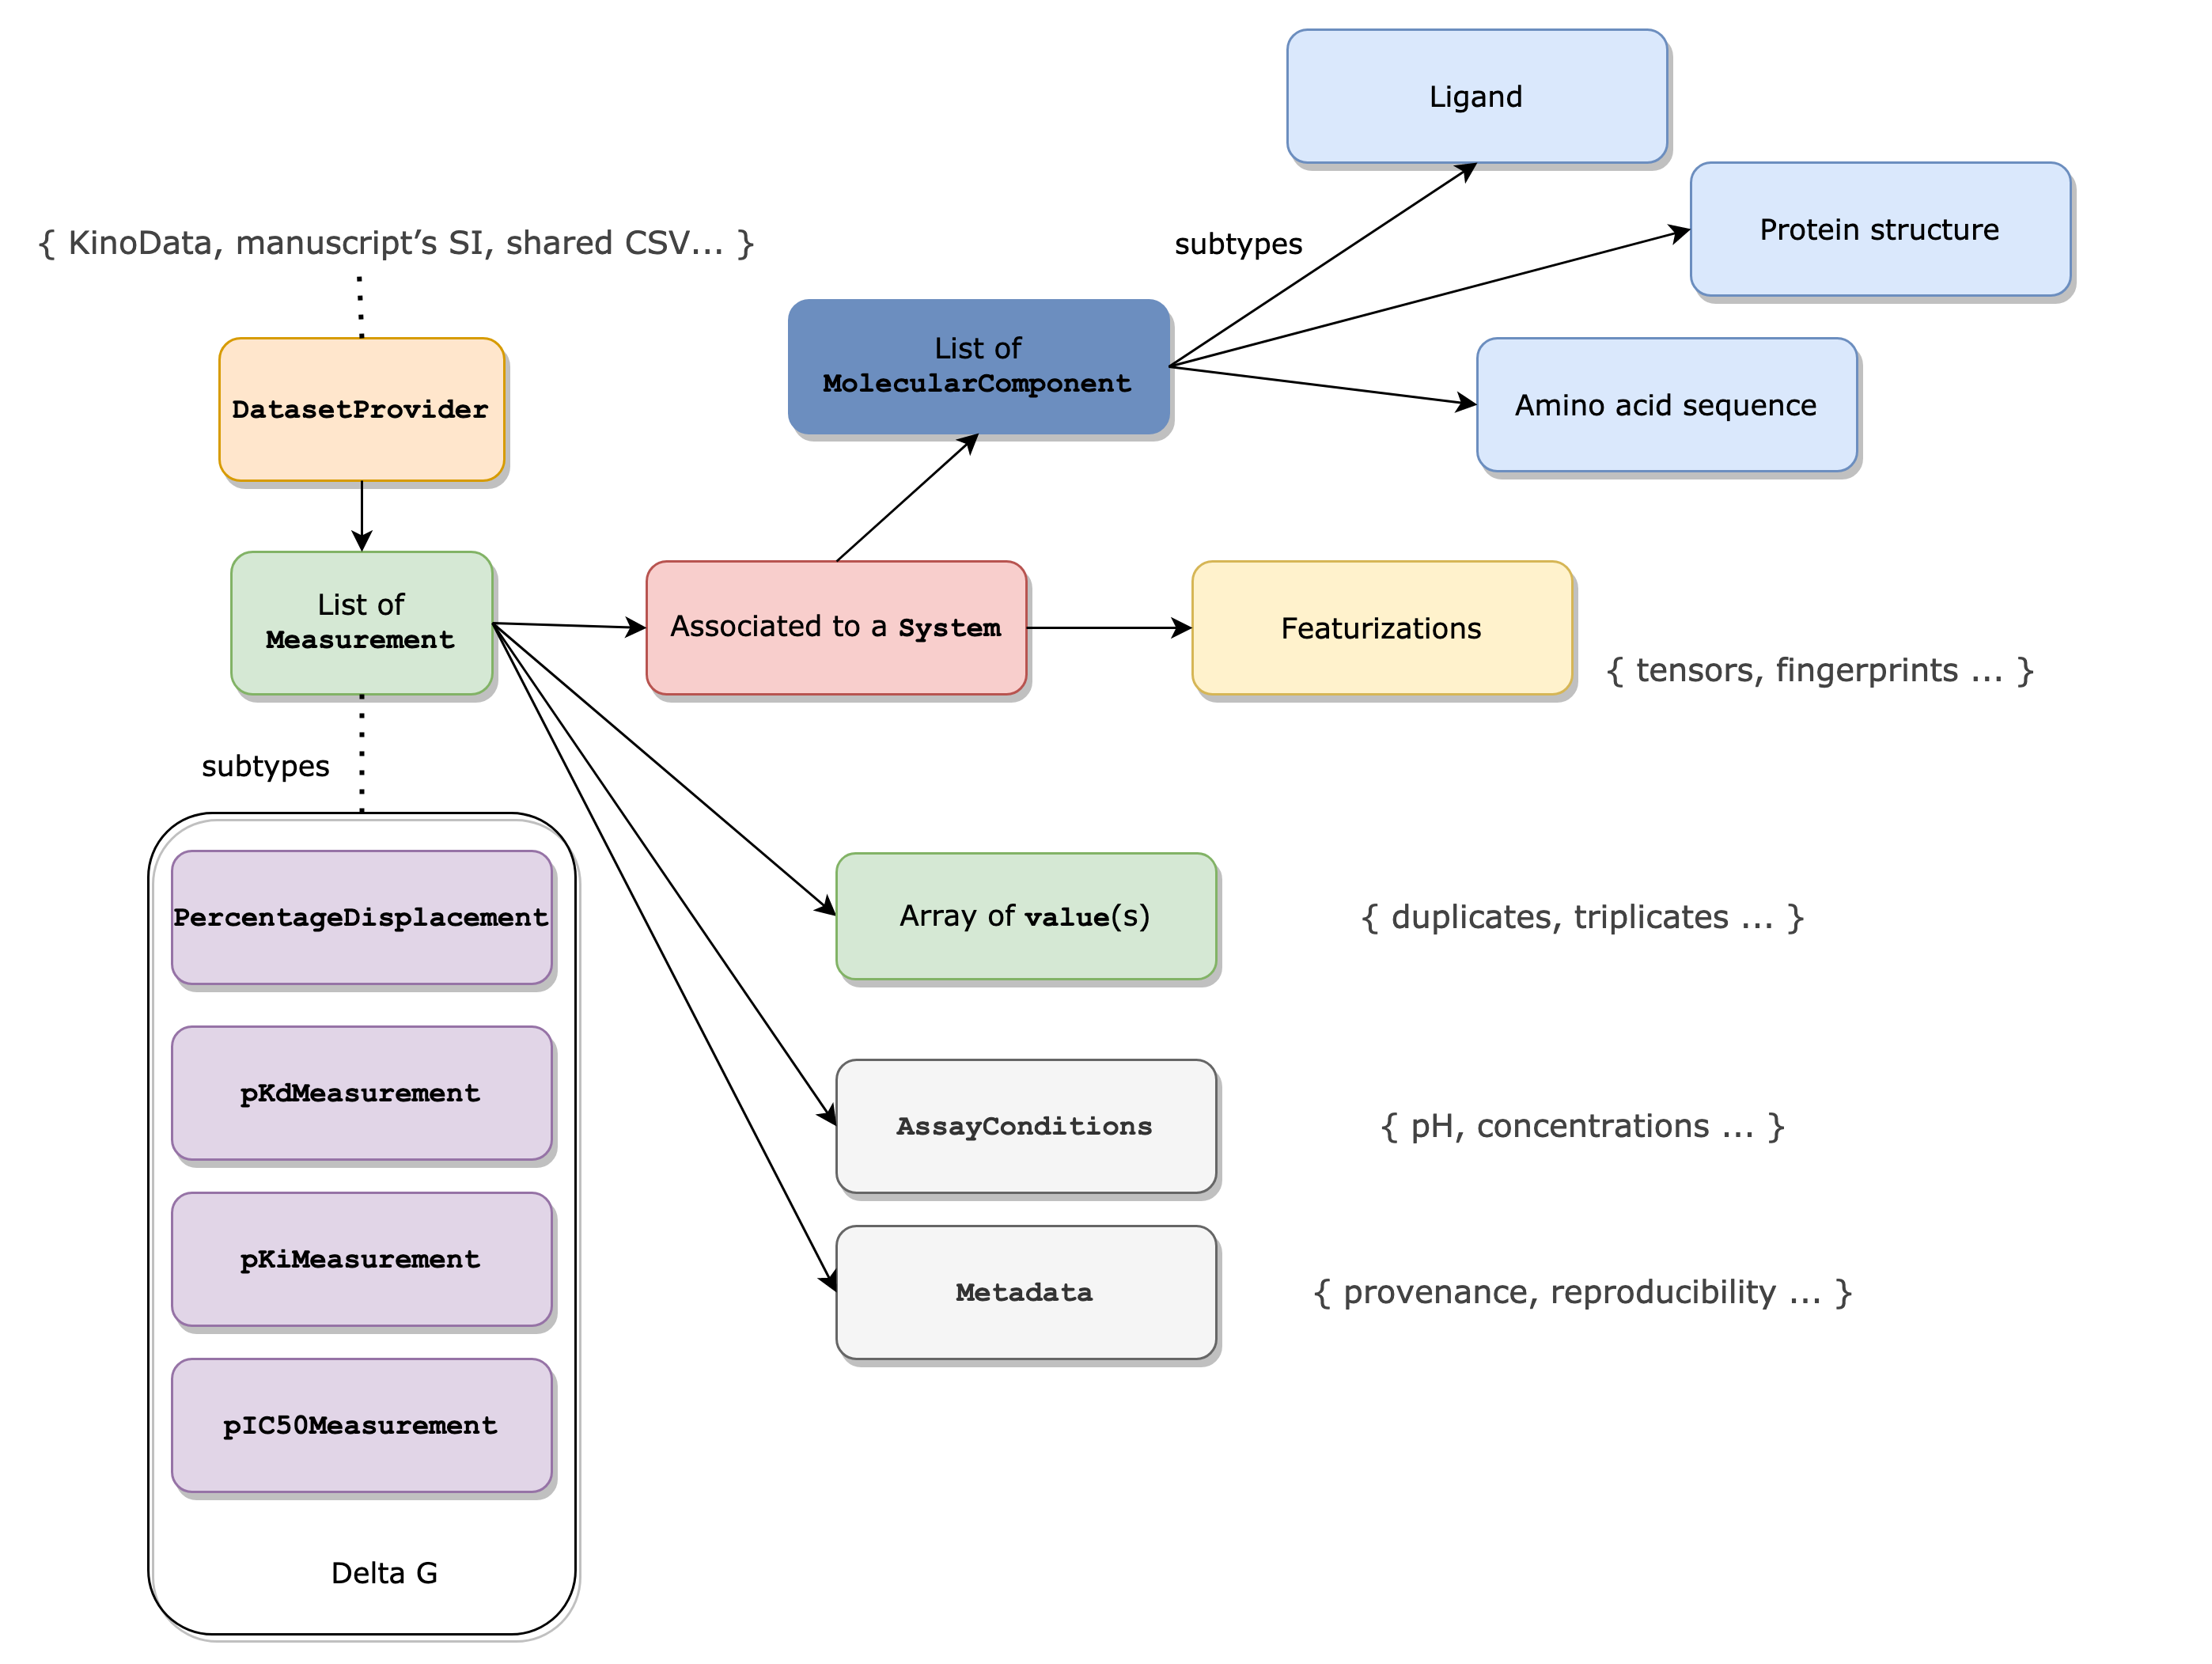
\includegraphics[width=0.5\linewidth]{figures/object_model.png}
\caption{\textbf{kinoml.core.} Add.}
\label{fig:object_model}
\end{figure}

\subsection{The challenges and the requirements}

For fair, reproducible and robust comparisons across different types of machine learning models, one needs to account for different sources of variability in the underlying data. The key challenges in this aspect are summarized below.

\subsubsection{Permanent access to the raw data}

The origin of the data is very important for reproducibility. The source and uniquely identifying tags need to be annotated and stored. Ideally, this means that the data is versioned and available via a unique resource address, such as a git tag or a DOI.

For example, Drewry's Published Kinase Inhibitor Set 2~(PKIS2) dataset can be downloaded from the Supporting Information~\cite{drewry_2017_PLOS}[S4 Table] attached to the corresponding manuscript~\cite{drewry_2017_PLOS}. Thanks to the associated DOI, the data can be traced back to its source.

Online web services such as ChEMBL~\cite{chembl_May_2021} contain a lot of data, a subset of which is incredibly useful for kinase-focused machine learning. The nature of these online resources is that they are updated constantly. Retrieving the useful bits can be automated in Python with the help packages such as \texttt{chembl\_webresource\_client}~\cite{chemblweb_May_2021}. However, ChEMBL in particular does not provide a way to version the acquisition: you will always obtain the latest data available. This means that the same query run twice, several days apart, might return different results. While ChEMBL does offer versioned database dumps~\cite{chemblarchives_May_2021}, these need to be downloaded first and then queried with SQL syntax.

To overcome these hurdles, we set up a project named KinoData. The repository \href{https://github.com/openkinome/kinodata}{openkinome/kinodata} governs the process of querying (and cleaning) wide purpose databases such as ChEMBL while guaranteeing its provenance and reproducibility through automated protocols. If new queries and curation protocols need to be added to the pipeline, a new release will be cut --see \href{https://github.com/openkinome/kinodata/releases/tag/v0.1}{openkinome/kinodata/releases/tag/v0.1}-- and the resulting artifact files (compressed CSV datasets) will be versioned and archived for posterity.

\subsubsection{From raw data to a unified object model}

One of the most useful types of data needed in the context of drug design is binding affinity, commonly noted $\Delta G$, which involves at least three elements: the measurement itself (one or more scalars), and two molecular counterparts (a protein or target, and a small compound or ligand). The relationship between measurements and molecules is a bit more nuanced than one might think:

\begin{enumerate*}[label=(\roman*)]
    \item The same ligand can be measured against several proteins.
    \item The same protein can be targeted with different ligands.
    \item A protein-ligand combination, which can be called a system or complex, can be measured once, several times under different conditions (different experiments), or even several times under the same conditions (replicates).
\end{enumerate*}

A the same time, data itself can come from very diverse sources, formatted in different ways. Among others: Excel spreadsheets, CSV files, PDF files, SQL databases, HTML tables, web applications. No matter the source, the data has to be funnelled into a \textit{unified object model} that is able to represent the observed measurements in a flexible yet concise way. If the aim is a sufficiently robust object model, any data conversions can be automated along the way. This process is governed by \texttt{kinoml.datasets}. The \texttt{kinoml.core} subpackage specifies the following object model and is illustrated in Figure~\ref{fig:object_model}:

\begin{enumerate}
    \item A \texttt{DatasetProvider} is essentially a list of \texttt{Measurement} objects.
    \item A \texttt{Measurement} is essentially a float (singlicate) or a list of floats (replicates), associated to a \texttt{System} plus some experimental conditions.
    \item A \texttt{System} is a list of \texttt{MolecularComponent} objects; usually a \texttt{Protein} and a \texttt{Ligand}.
    \item \texttt{MolecularComponent} objects can be of very different nature, depending on how the raw data for that molecular entity is encoded.
\end{enumerate}

\subsubsection{Molecular components, representations and entities}
Published datasets do not often provide information about what was measured exactly. They will contain enough data to identify the intent, but maybe not enough to reconstruct the experimental conditions in a computational workflow. For example, information about the measured proteins might be encoded via:

\begin{enumerate*}[label=(\roman*)]
    \item The corresponding gene names, without necessarily mentioning possible mutations, PTMs or splicing variants,
    \item the UniProt identifier,
    \item the FASTA sequence,
    \item a PDB identifier.
\end{enumerate*}

Ligands might be encoded with:

\begin{enumerate*}[label=(\roman*)]
    \item IUPAC names,
    \item (Non-canonical) SMILES~\cite{weininger_1988_JChemInfComputSci},
    \item InChI keys~\cite{heller_2013_JCheminform}, or
    \item SDF files
\end{enumerate*}

(see Figure~\ref{fig:kinodata}). However, the molecule representations should not be encoding-dependent, since they refer to the same underlying molecular entity. Therefore, the constructed object model must be able to account for that. We strive to provide an object model that can funnel all these different molecular representations into the same idealized representation of the molecular entity. Notice we mention the possibility, not the requirement. Some workflows do not need to go through the expensive demands of constructing a fully-fledged \texttt{Protein} object out of a PDB identifier, and hence spare time and memory if the dataset contains enough information for the needs of the experiment. That does not mean that the workflow is not reproducible: in the end, a part of the object model tree was used to annotate the objects with sufficient provenance information.

More details are available at \href{http://openkinome.org/kinoml/api/core/components/}{http://openkinome.org/kinoml/api/core/components/}.

\subsubsection{Measurement types and uncertainties}

Most experimental assays do not estimate $\Delta G$ of binding directly, but proxy measurements such as $IC_{50}$, $K_d$, $K_i$, or percentage of displacement. Additionally, those assays are performed by different laboratories with different protocols and techniques. This all leads to different experimental uncertainties and soft measurements. While the data can be noisy, it is definitely informative and has the potential to provide predictive power in an adequately tuned model.
This results in the following requirements:

\begin{enumerate}
    \item The framework must handle different measurement types that, nonetheless, represent the same underlying physical phenomenon $\Delta G$.
    \item To leverage several measurement types in the same learning exercise, the models will be instructed to learn $\Delta G$. Since the losses are computed against the observed measurement (e.g. $IC_{50}$), this calls for mathematical expressions that maps the two. As such, each measurement type features its own observation model.
    \item For the sake of reproducibility, each measurement needs to be annotated with provenance data (source dataset, publication,...).
    \item To combine different sources of data, measurements need to contain information about the uncertainty. When this is not available, it can be estimated or learned.
\end{enumerate}

More details are available at \href{http://openkinome.org/kinoml/api/core/measurements/}{http://openkinome.org/kinoml/api/core/measurements/}.


% JRG: At this point we haven't talked about featurization yet, but we do talk about it like a familiar concept in the coming sections. Maybe we need to write something about it beforehand.


\subsubsection{The software}

Achieving these goals and fulfilling these requirements require modular libraries that allow us to compose the needed pipelines.
Mention Deepchem~\cite{Ramsundar_2019_deepchem}?
\begin{figure}
\centering
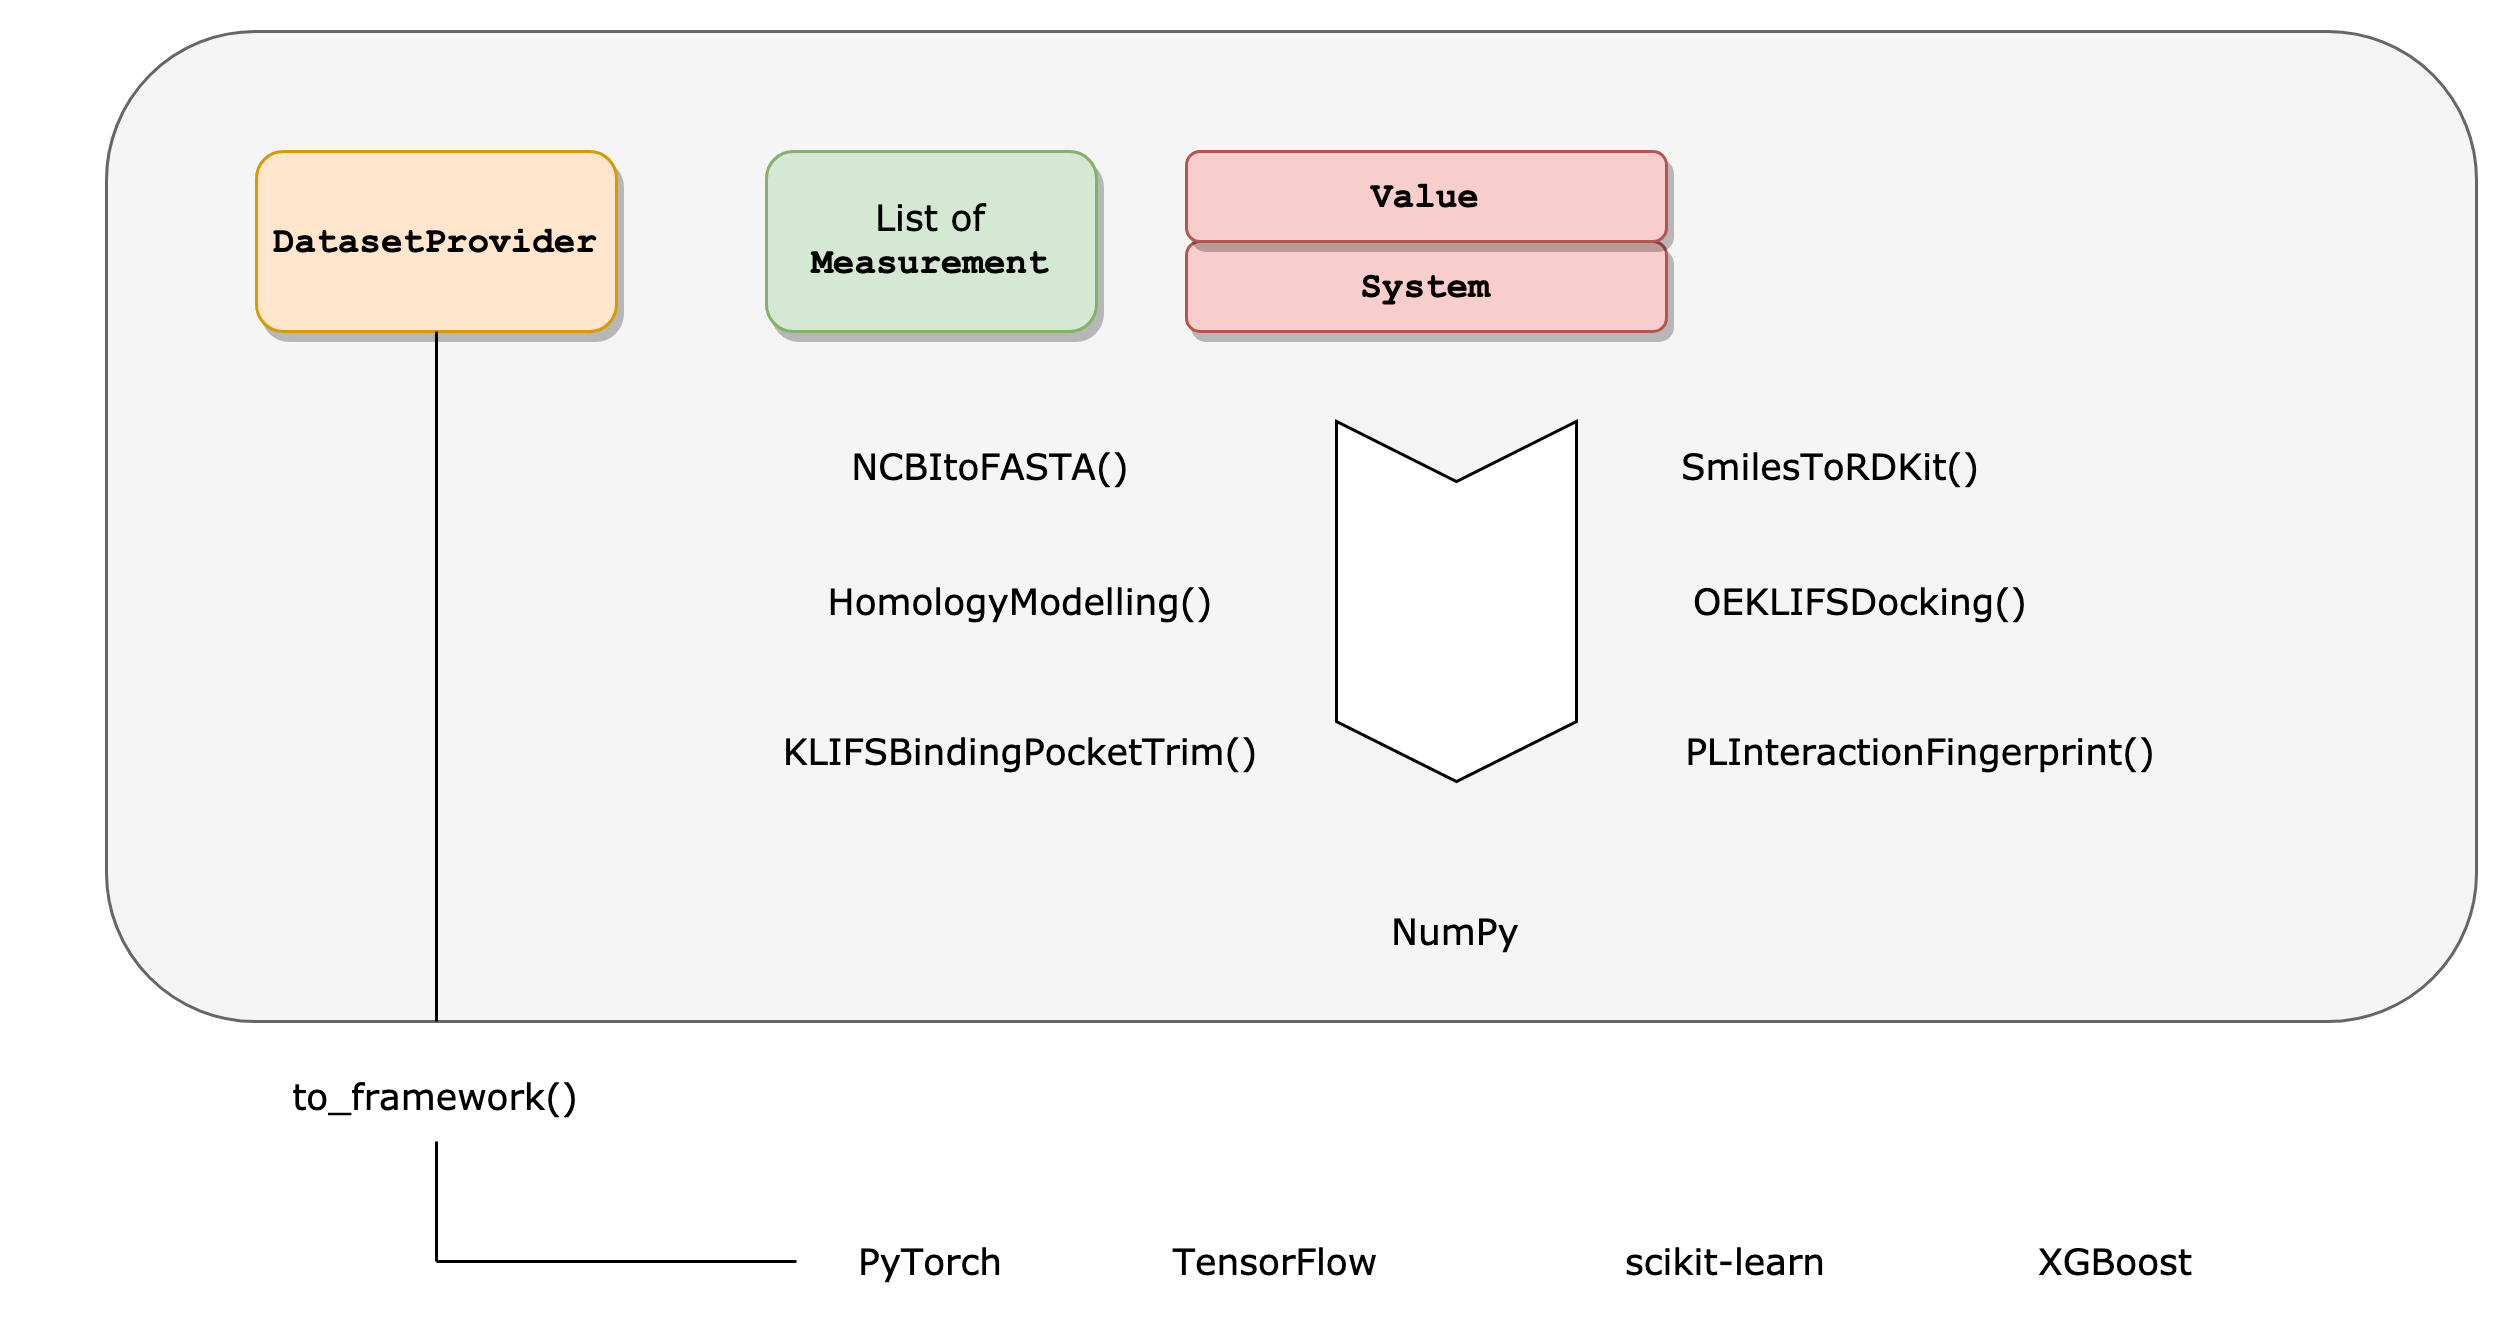
\includegraphics[width=0.5\linewidth]{figures/ml_frameworks.png}
\caption{\textbf{Machine learning frameworks.}}
\label{fig:ml_frameworks}
\end{figure}

Our main library is \href{https://github.com/openkinome/kinoml/}{openkinome/kinoml}. It provides all the building blocks at the different stages of the pipeline. Some highlights:

\begin{itemize}
    \item Data ingestion is done at \texttt{kinoml.datasets}.
    \item The unified object model is specified at \texttt{kinoml.core}.
    \item  The different elements of the featurization pipelines can be found at \texttt{kinoml.features}.
    \item Machine learning models are provided in \texttt{kinoml.ml}. This subpackage also provides tooling to juggle different machine learning backends, such as Numpy~\cite{harris_2020_nature}, PyTorch~\cite{paszke_2019_neurips}, scikit-learn~\cite{scikit-learn, sklearn_api} or XGBoost~\cite{chen_2016_xgboost}, see Figure~\ref{fig:ml_frameworks}.
\end{itemize}

The result-oriented pipelines are built in additional repositories, prefixed with experiments-*. For example, \href{https://github.com/openkinome/experiments-binding-affinity}{https://github.com/openkinome/experiments-binding-affinity} provides an automated notebook running system based on templates and papermill~\cite{papermill_May_2021}. It encourages separating featurization from training by design, so the same tensors can be reused across different models. Additionally, the same models can be trained with different featurization schemes.

Finally, providing curated data ready to be ingested at \texttt{kinoml} is tackled by \texttt{openkinome/kinodata}\href{https://github.com/openkinome/kinodata}. Here, several notebooks query different online resources to obtain an updated list of the human kinome and the presence of relevant bioactivity in different datasets, such as ChEMBL. CSV artifacts are released on GitHub and downloaded, and cached by \texttt{kinoml.datasets} during featurization.

\subsubsection{The team}

The OpenKinome initiative is the product of an ongoing collaboration between \href{https://volkamerlab.org/}{Volkamer lab} (Berlin, DE) and \href{https://www.choderalab.org/}{Chodera lab} (New York, USA).

%\subsection{API}

% JRG: I think we have covered the essential aspects of the API above. 

%\subsubsection{kinoml object model}

% JRG: I think we have covered the essential aspects of the API above. 

%\subsubsection{Delegation to ML frameworks}

% JRG: This will be covered in the missing "Featurization" section mentioned above.

%\subsubsection{Reproducibility}

% JRG: This is partially addressed in the "Software" subsection.

%\section{Results}

% JRG: Discuss what are we trying to present here. The libraries? The concepts?

%\section{Discussion}

% JRG: Reflect on the challenges and the proposed strategies to deal with them. Laying down the foundational framework to support these ideas is time-consuming and very sensitive to which initial choices are made. Tell the community that these things _are_ important and maybe mention a couple of lessons learned.

%%%%%%%%%%%%%%%%%%%%%%%%%%%%%%%%%%%%%%%%%%%%%%%%%%%%%%%%%%%%%%%%%%%%%%%%%%%%%%%%%%%%%%%%%%%%%%%%%%%%%%
% Code and Data Availability
%%%%%%%%%%%%%%%%%%%%%%%%%%%%%%%%%%%%%%%%%%%%%%%%%%%%%%%%%%%%%%%%%%%%%%%%%%%%%%%%%%%%%%%%%%%%%%%%%%%%%%

\section{Code and data availability}
Code is available at \href{https://github.com/openkinome}{https://github.com/openkinome}.


%%%%%%%%%%%%%%%%%%%%%%%%%%%%%%%%%%%%%%%%%%%%%%%%%%%%%%%%%%%%%%%%%%%%%%%%%%%%%%%%%%%%%%%%%%%%%%%%%%%%%%
% Author Contributions 
%%%%%%%%%%%%%%%%%%%%%%%%%%%%%%%%%%%%%%%%%%%%%%%%%%%%%%%%%%%%%%%%%%%%%%%%%%%%%%%%%%%%%%%%%%%%%%%%%%%%%%
\section{Author Contributions}

(Follow the \href{http://www.cell.com/pb/assets/raw/shared/guidelines/CRediT-taxonomy.pdf}{CRediT Taxonomy})

%%%%%%%%%%%%%%%%%%%%%%%%%%%%%%%%%%%%%%%%%%%%%%%%%%%%%%%%%%%%%%%%%%%%%%%%%%%%%%%%%%%%%%%%%%%%%%%%%%%%%%
% Acknowledgments 
%%%%%%%%%%%%%%%%%%%%%%%%%%%%%%%%%%%%%%%%%%%%%%%%%%%%%%%%%%%%%%%%%%%%%%%%%%%%%%%%%%%%%%%%%%%%%%%%%%%%%%
\section{Acknowledgments}
Funded by \href{https://www.stiftung-charite.de/}{Stiftung Charité}, \href{https://www.einsteinfoundation.de/en/people-projects/einstein-bih-visiting-fellows/john-chodera/}{Einstein BIH Visiting Fellow Project}, Bayer AG, and others.

%%%%%%%%%%%%%%%%%%%%%%%%%%%%%%%%%%%%%%%%%%%%%%%%%%%%%%%%%%%%%%%%%%%%%%%%%%%%%%%%%%%%%%%%%%%%%%%%%%%%%%
% Disclosures 
%%%%%%%%%%%%%%%%%%%%%%%%%%%%%%%%%%%%%%%%%%%%%%%%%%%%%%%%%%%%%%%%%%%%%%%%%%%%%%%%%%%%%%%%%%%%%%%%%%%%%%
\section{Disclosures}

JDC is a member of the Scientific Advisory Board for Schr\"{o}dinger, LLC.

\section{Abbreviations}
List of abbreviations used in the paper.
\begin{table}[H]
    \centering
    \begin{tabular}{l l}
        DOI & Digital Object Identifier \\
        CSV & Comma-Separated Values\\
        PTM & Post-Translational Modification \\
        IUPAC & International Union of Pure and Applied Chemistry \\
        SMILES & Simplified Molecular-Input Line-Entry System \\
        InChI & International Chemical Identifier \\
        SDF & Structure-Data File \\
        PDB & Protein Data Bank \\
    \end{tabular}
    %\caption{Caption}
    %\label{tab:my_label}
\end{table}

\nocite{*} % This command displays all refs in the bib file. PLEASE DELETE IT BEFORE YOU SUBMIT YOUR MANUSCRIPT!
\bibliography{bibliography}

%%%%%%%%%%%%%%%%%%%%%%%%%%%%%%%%%%%%%%%%%%%%%%%%%%%%%%%%%%%%
%%% APPENDICES
%%%%%%%%%%%%%%%%%%%%%%%%%%%%%%%%%%%%%%%%%%%%%%%%%%%%%%%%%%%%

\appendix


\end{document}
